\documentclass[a4paper,11pt] {article}
% Default margins are too wide all the way around. I reset them here
\setlength{\topmargin}{.5in}
\setlength{\textheight}{9in}
\setlength{\oddsidemargin}{.125in}
\setlength{\textwidth}{6.25in}

\usepackage{color}
\usepackage{listings}
\usepackage[utf8]{inputenc}
\usepackage{graphicx}
\usepackage{float}
\usepackage{pdfpages}
\usepackage{amsthm}
\usepackage{amsmath,amsfonts,amssymb,amsthm}
\theoremstyle{definition}
\newtheorem{defn}{Definition}[section]
\newtheorem{conj}{Conjecture}[section]
\newtheorem{exmp}{Example}[section]

\definecolor{javared}{rgb}{0.6,0,0} % for strings
\definecolor{javagreen}{rgb}{0.25,0.5,0.35} % comments
\definecolor{javapurple}{rgb}{0.5,0,0.35} % keywords
\definecolor{javadocblue}{rgb}{0.25,0.35,0.75} % javadoc
 \usepackage[french]{babel}
\usepackage[T1]{fontenc}
\lstset{language=Java,
basicstyle=\ttfamily,
keywordstyle=\color{javapurple}\bfseries,
stringstyle=\color{javared},
commentstyle=\color{javagreen},
morecomment=[s][\color{javadocblue}]{/**}{*/},
numbers=left,
numberstyle=\tiny\color{black},
stepnumber=2,
numbersep=10pt,
tabsize=4,
showspaces=false,
showstringspaces=false}

\lstset{
language=R,
basicstyle=\scriptsize\ttfamily\color{javadocblue},
commentstyle=\ttfamily\color{javagreen},
numbers=left,
numberstyle=\ttfamily\color{javagreen}\footnotesize,
stepnumber=1,
numbersep=5pt,
backgroundcolor=\color{white},
showspaces=false,
showstringspaces=false,
showtabs=false,
frame=single,
tabsize=2,
captionpos=b,
breaklines=true,
breakatwhitespace=false,
title=\lstname,
escapeinside={},
keywordstyle={},
morekeywords={}
}

\begin{document}
\title{\textbf{Usability \& Skeuomorphism}}
\author{\textbf{Bodart Xavier} - \textbf{Chapeaux Thomas} - \textbf{Mayeur Bernard} \\
Université Libre de Bruxelles}

\maketitle
\begin{center}

\textbf{INFO-F501 Information technology in society\\
Luc WILKIN}
\end{center}
\begin{center}


\includegraphics[scale=0.15]{ULBjea.jpg} 
\end{center}
\pagebreak
\tableofcontents
\pagebreak
\section{Introduction}
\section{Theoretical concepts \& design principles}
\subsection{Perceived affordance}
Perceived affordance represents the quality of an object to suggest its utilization. This concept is quite important in object-design due to the fact that it may represents the main source of information about the usage of the object. Indeed, people tends to read less and less the usage notice. In addition, this concept may reinforce the feeling of experience of a person for a given object.
\begin{figure}[h]
\centering
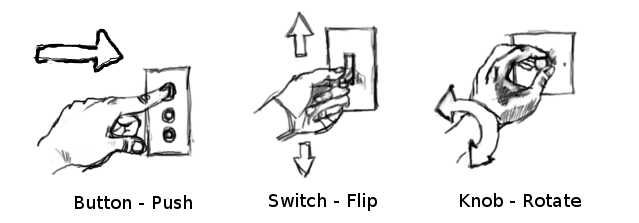
\includegraphics[scale=0.40]{switches-only.png}
\caption{By their forms, buttons,switches or knobs often suggest their working.}
\end{figure}

An important thing to notice is the fact that perceived affordance is not always the same as real affordance.
Indeed, design can rarely explain the complete working of some complex object. The perceived affordance is only capable to show primitive properties about the usage of an object. Furthermore, a bad design may induce a more difficult usage than the correct one.%http://www.interaction-design.org/encyclopedia/affordances.html
\begin{figure}[h]
\centering
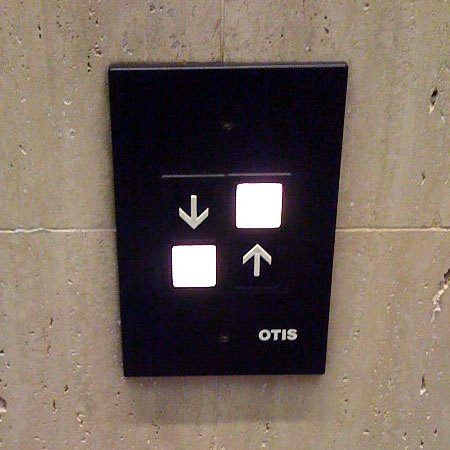
\includegraphics[scale=0.20]{bad-switches.jpg}
\caption{What would you do in front of such lift panel?}
\end{figure}
\subsection{Natural mapping}
Natural mapping is a concept that suggest to organize controllers in the same arrangement as the objects on which they have an influence to guarantee the expected result. This principle will often lead to an increasing of perceived affordance.\\

A common example to illustrate such concept is the placement of the buttons that control the different stoves of your kitchen.It's obvious that the most left-top button will regulate the temperature of the most left-top stove.\\
 \begin{minipage}{\linewidth}
      \centering
      \begin{minipage}{0.45\linewidth}
          \begin{figure}[H]
          \centering
              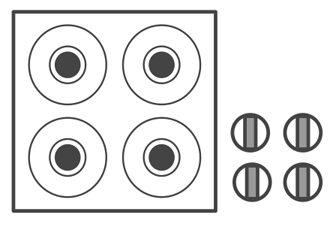
\includegraphics[scale=0.3]{stove_natural.png}
              \caption{Scheme of a four stoves set with their corresponding knobs}
          \end{figure}
      \end{minipage}
      \hspace{0.05\linewidth}
      \begin{minipage}{0.45\linewidth}
          \begin{figure}[H]
                    \centering
              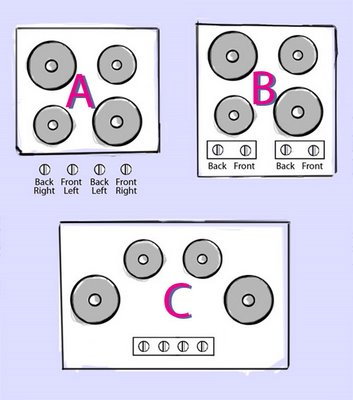
\includegraphics[scale=0.4]{NormanBurners.jpg}
              \caption{These designs are eligible if you have the same assumption as the producer}
          \end{figure}
      \end{minipage}
  \end{minipage}
  \bigskip
  
  
Unfortunately, such principle may sometimes induce extra-design cost and may also depends on the point of view of the producer: Even if it seems logical for certain arrangement such stoves or the control of the electronic windows of the car, One can still doubt about the mapping of light switches(\textit{"Does this switch controls  the lights of the front of the room because it is above the others ?"}). %http://karikariboberry.blogspot.be/2008/09/natural-mapping.html
\subsection{Feedback}
\newtheorem{mydef}{Definition}
\begin{mydef}
\textit{\textbf{Feedback}} is the return of a fraction of the output signal from an amplifier, microphone, or other device to the input of the same device; sound distortion produced by this.%http://www.oxforddictionaries.com/definition/english/feedback
\end{mydef}

In our case, feedback represents any action that could indicate to the user that its interaction with the item was taken into account.



\subsection{Constraints}
\subsubsection{Physical constraints}
\subsubsection{Logical constraints}
\subsubsection{Cultural constraints}
\subsubsection{Semantic constraints}
\subsection{Skeuomorphism}
\subsection{Flat design}

\section{Evolution of the computer-interface}
\subsection{Command line interpreter}
\subsection{Graphical interface \& computer mouse}
\subsection{Touch interface}
\subsection{Voice interface}
\subsection{Neural interface}
\section{Experiment}
\subsection{Definition of the experiment}
\subsection{Results analysis}
\subsection{Comparison with previous studies}
\section{Conclusion}
%Bibliography
\end{document}